\documentclass[xcolor=dvipsnames, 14pt]{beamer}

\usepackage{beamerthemesplit}
\usepackage[mathscr]{eucal}
\usepackage{pgfpages}
\usepackage{graphicx}
\graphicspath{ {c:/Users/Marissa/} }

\usepackage{comment}
\usepackage{hyperref}
\usepackage{import}
\usepackage{amsmath, amsfonts, amscd, amssymb}
\usepackage{epsfig}
\usepackage{graphicx}
\usepackage{url}
\usepackage{mathrsfs}
\usepackage{makeidx}
\usepackage{color}
\usepackage{verbatim}
\usepackage{listings}
\usepackage{multicol}
\usepackage{algorithmicx}
\usepackage[plain]{algorithm}
\usepackage[noend]{algpseudocode}
\usepackage{float}
\usepackage{paralist}
\usepackage{caption}
\usepackage{subcaption}
\usepackage{textcomp}
\usepackage[framemethod=tikz]{mdframed}
\usepackage{tikz}
\usetikzlibrary{shapes,arrows, automata, backgrounds, calendar, chains, decorations,
	matrix, mindmap, patterns, petri, positioning, shadows, shapes.geometric,
	trees}
\definecolor{boxbackground}{rgb}{1,0.976,0.882}

\lstset{
language=Python,
basicstyle=\ttfamily\scriptsize,
keywordstyle=\color{blue}\ttfamily,
stringstyle=\color{red}\ttfamily,
commentstyle=\color{green!50!black}\ttfamily,
frame=single,
breaklines=true,
postbreak=\raisebox{0ex}[0ex][0ex]{\ensuremath{\color{violet}\hookrightarrow\space}},
backgroundcolor = \color{boxbackground},
showspaces=false,
showstringspaces=false,
}


\usepackage{mathtools}

\defbeamertemplate{section page}{mine}[1][]{
  \vspace*{\fill}
  \begin{centering}
    \begin{beamercolorbox}[sep=12pt,center]{part title}
      \usebeamerfont{section title}\insertsection\par
    \end{beamercolorbox}
  \end{centering}
  \vspace*{\fill}
}

\setbeamertemplate{section page}[mine]

\setbeamertemplate{footline}
{
  \leavevmode%
  \hbox{%
  \begin{beamercolorbox}[wd=.7\paperwidth,ht=2.25ex,dp=1ex,center]{author in head/foot}%
    \usebeamerfont{author in head/foot}{}
  \end{beamercolorbox}%
  \begin{beamercolorbox}[wd=.3\paperwidth,ht=2.25ex,dp=1ex,center]{title in head/foot}%
    \usebeamerfont{title in head/foot}{}
  \end{beamercolorbox}%
  }%
  \vskip0pt%
}

\usefonttheme[onlymath]{serif}
\usetheme{Madrid}
%Options: default, albatross, beaver, beetle, crane, dolphin, dove, fly, lily, orchid, rose, seagull, seahorse, whale, wolverine
%Crane is orange, fly is ugly, albatross is bad, dolphin ditches colorboxes, beaver is red on gray, beetle is gray background
%dove is straight up black on white, lily ditches colorboxes, whale is normal, seahorse is a light blue
\usecolortheme{seahorse}
\setbeamertemplate{navigation symbols}{} 
\setbeamertemplate{items}[square] 
\setbeamertemplate{table of contents}[square]
\setbeameroption{hide notes}


\title[]{Predicting Fake News on Facebook}
\author[Marissa Graham]{Marissa Graham}
\institute{CS 401R Final Project}
\date{}

\begin{document}
\frame{\titlepage}

\begin{frame}{Motivation}
\centering

\includegraphics[width=10cm,height=6cm]{fake_news_collage.png}

\footnotesize
\begin{itemize}
\item Fake news has become more prevalent in U.S. politics.
\item Democracy can't work unless citizens have accurate information.
\end{itemize}
\end{frame}

\begin{frame}{Dataset}
\vspace{0.5cm}
\small
Being able to predict/flag fake news with some amount of accuracy using machine learning tools is helpful.
\vspace{0.25cm}

Dataset used:
\small
\begin{itemize}
\item Sponsored by Buzzfeed
\item 2284 Facebook posts from nine different news outlet pages (three left-wing, three right-wing, three mainstream) between 9/19/2016 and 9/27/2016, classified by accuracy level
\item Relevant features: 
\begin{itemize}
\footnotesize
\item \texttt{Category} (mainstream, right, or left)
\item \texttt{Page}
\item \texttt{Post Type} (video, link, text, photo)
\item \texttt{Rating} (mostly false, mostly true, mixture of true and false, no factual content)
\end{itemize}
\end{itemize}

\end{frame}

\begin{frame}
\centering
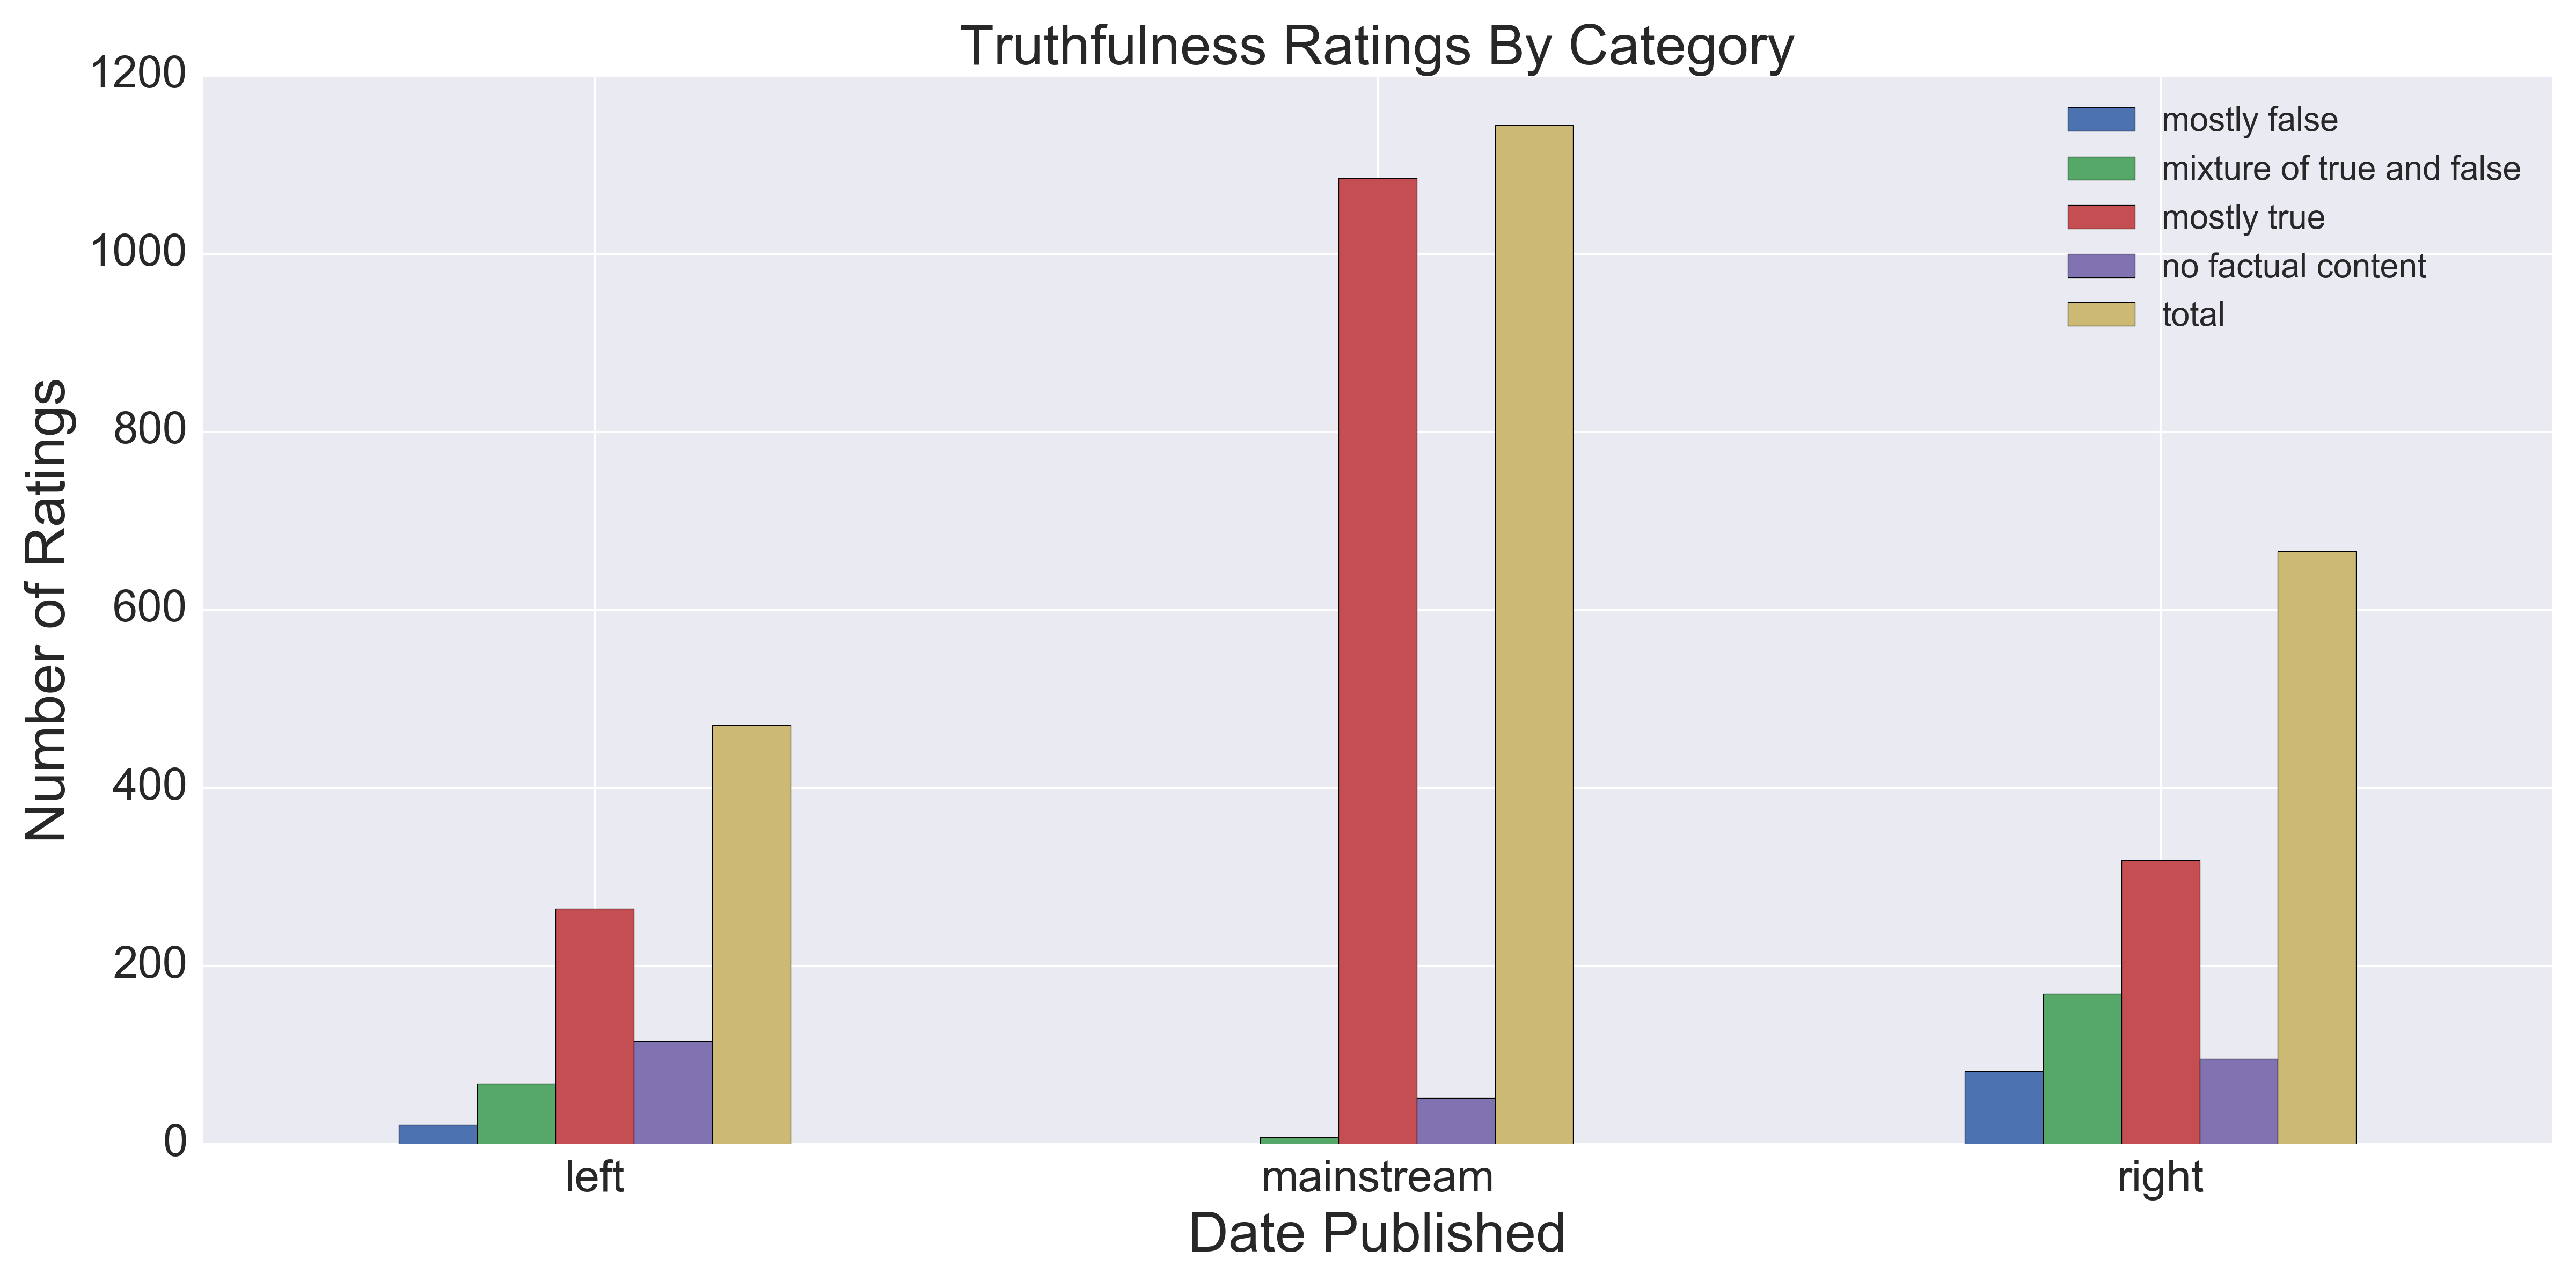
\includegraphics[width=12cm,height=7cm]{ratings_distribution_by_category.png}
\end{frame}

\begin{frame}
\centering
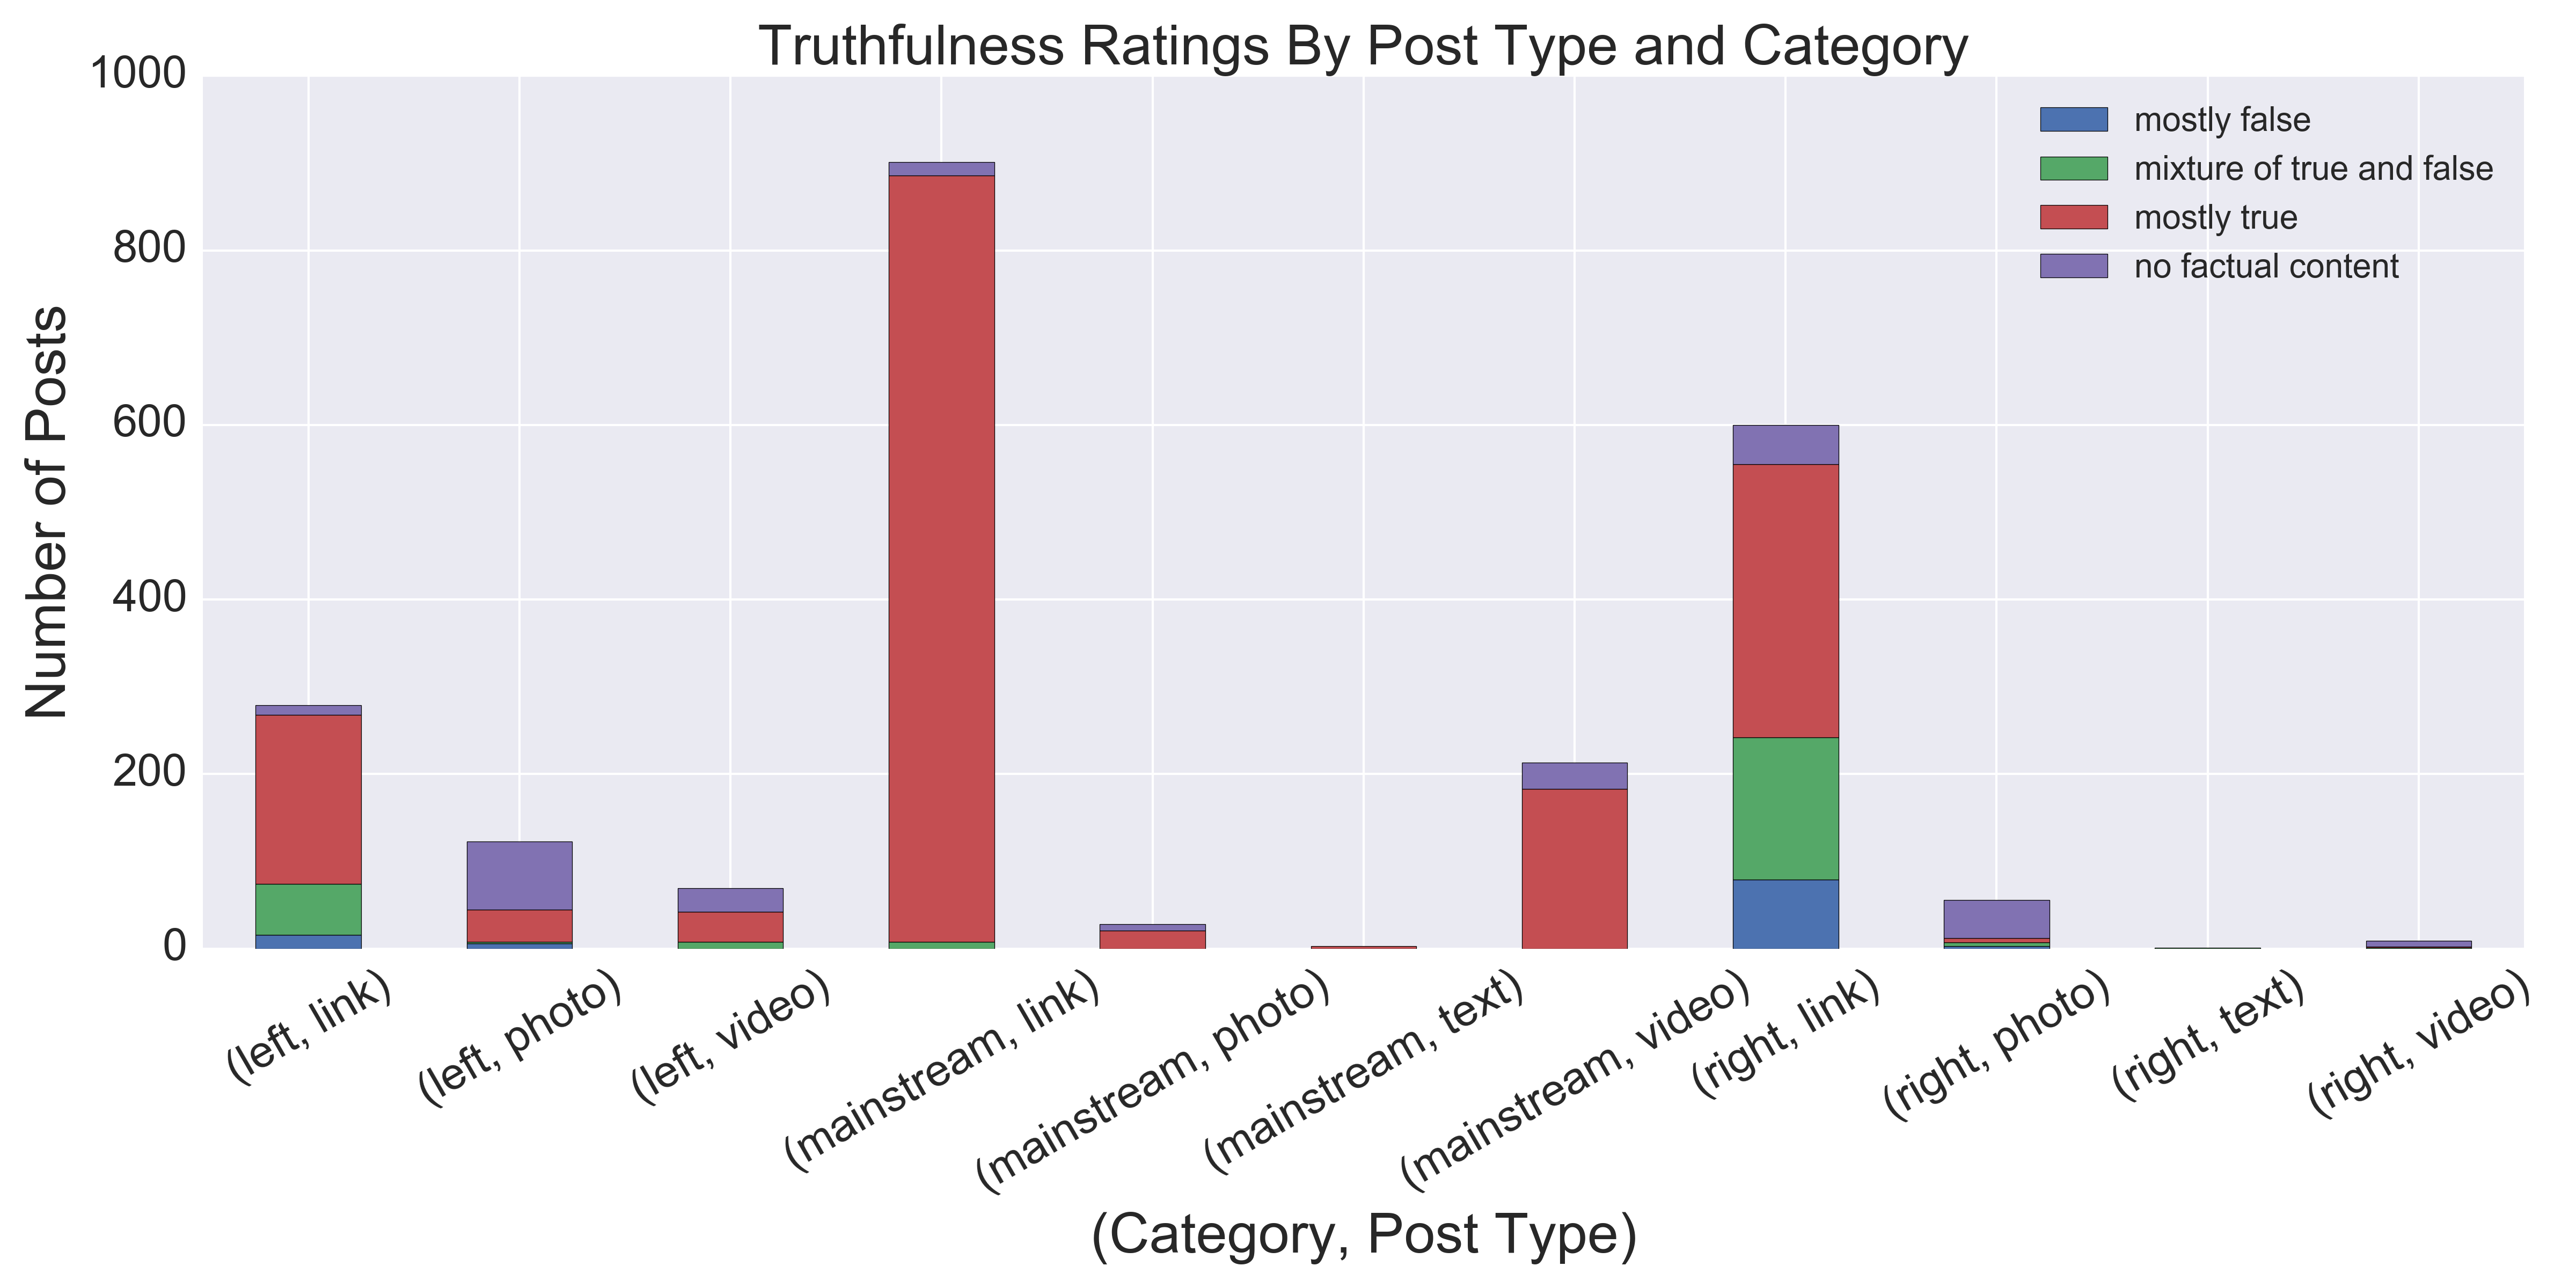
\includegraphics[width=6cm,height=4.5cm]{ratings_distribution_by_category_type.png}

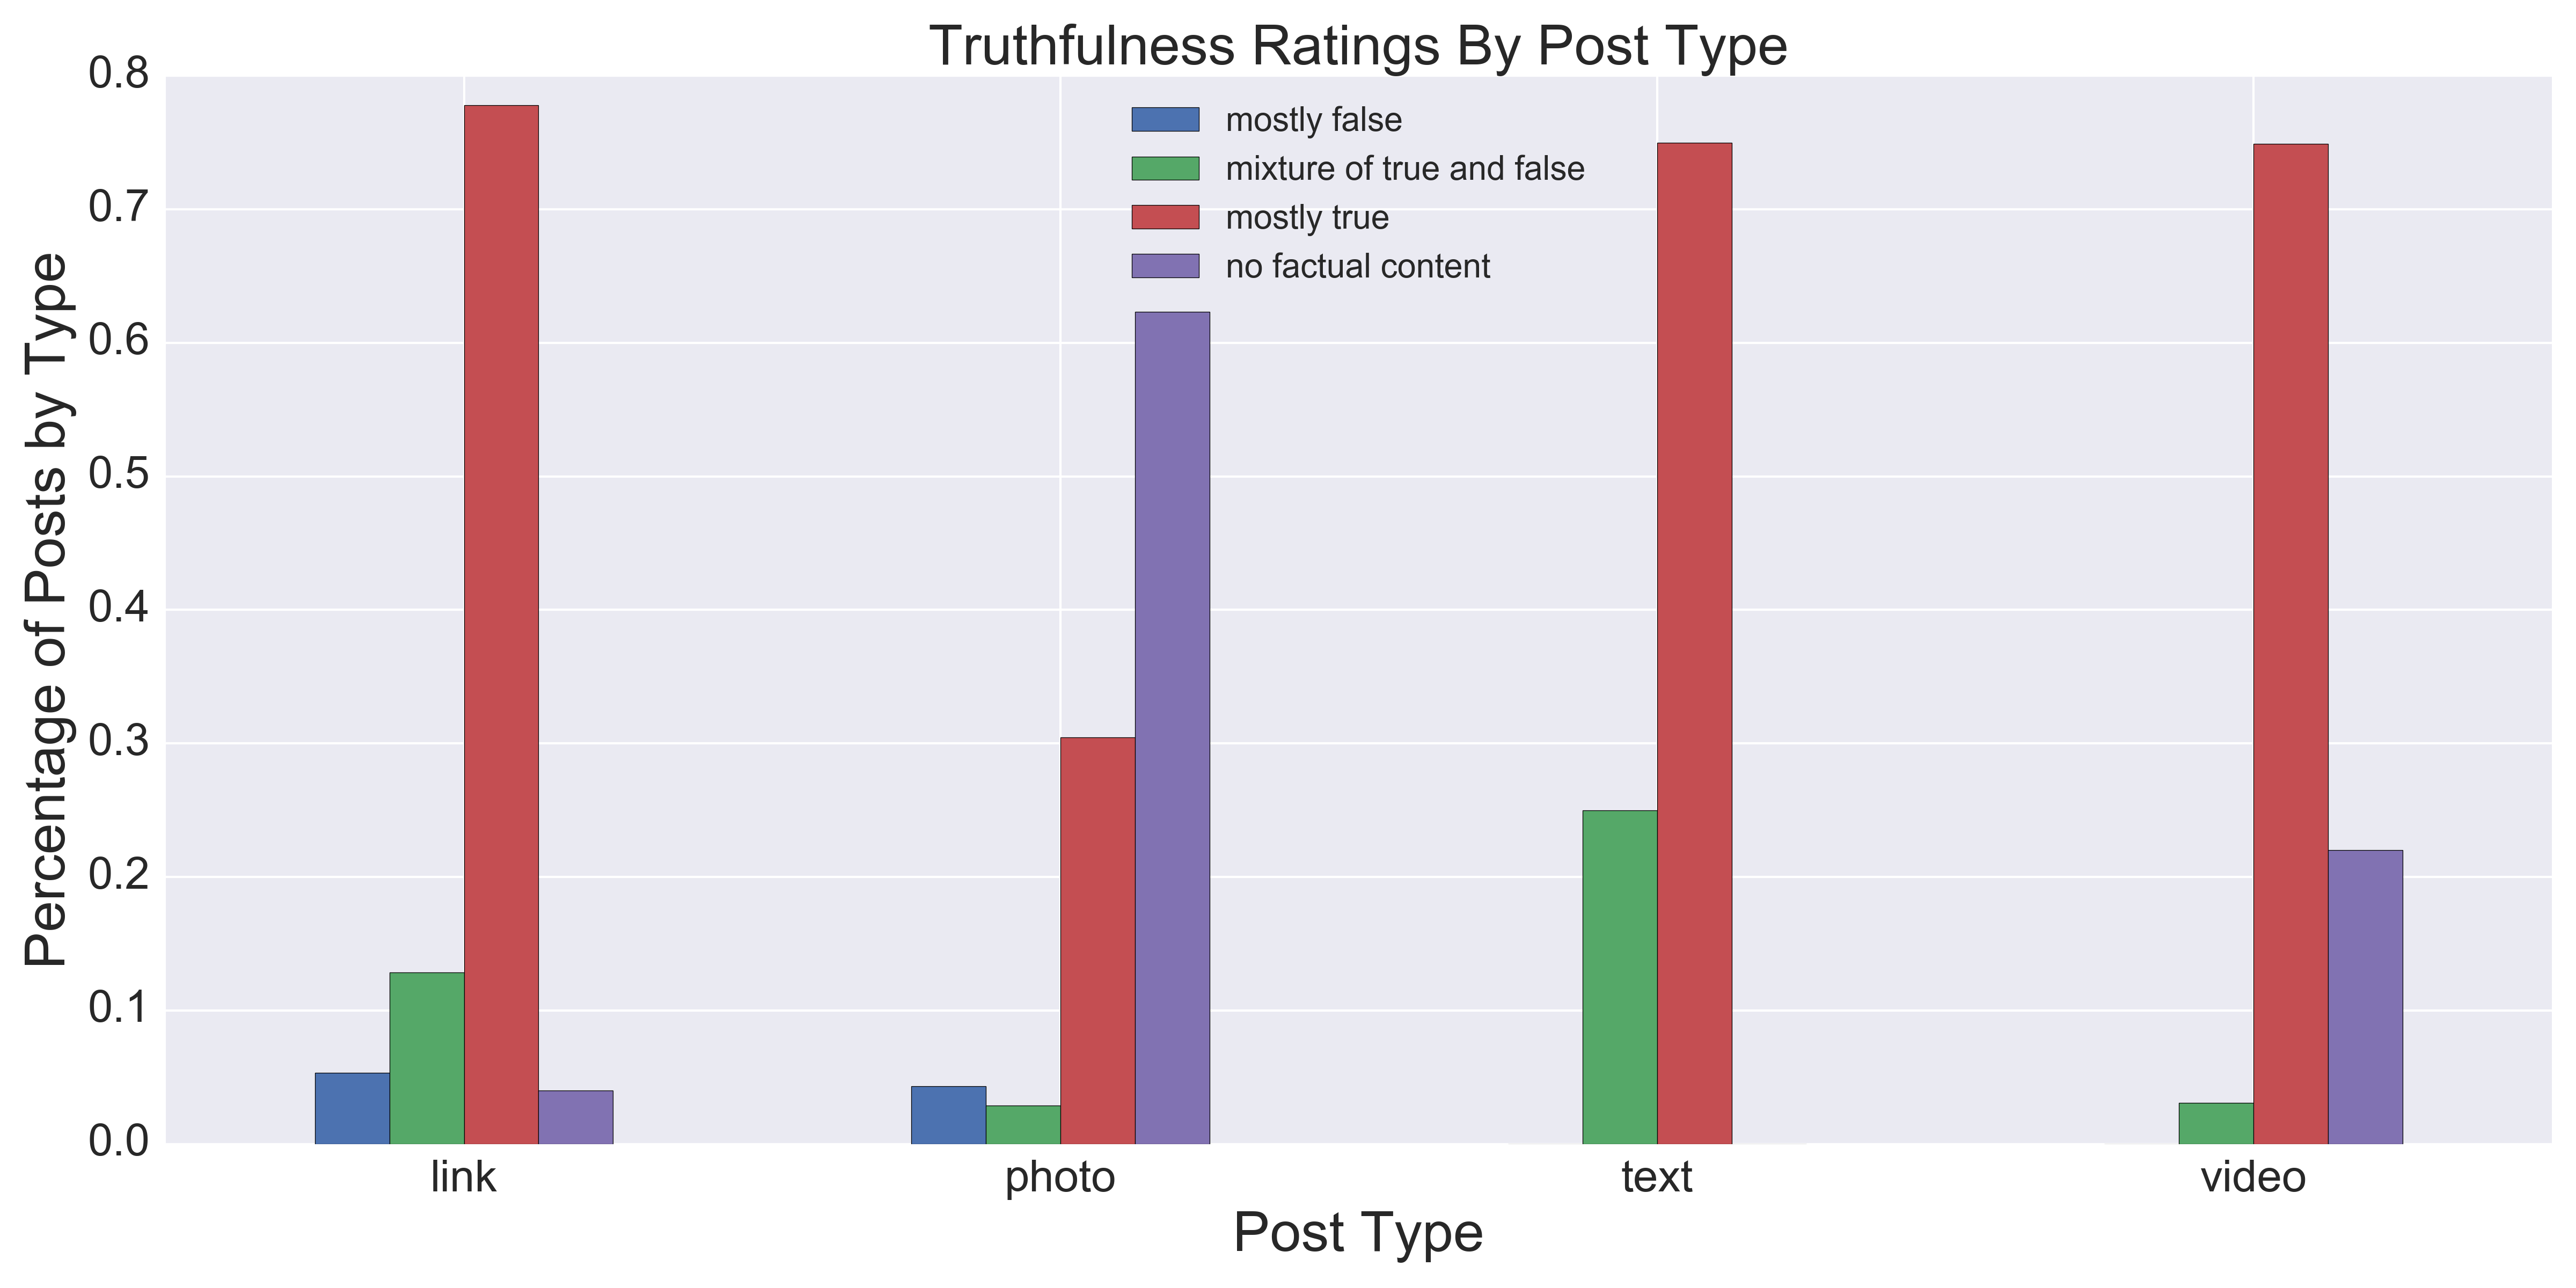
\includegraphics[width=6cm,height=3.5cm]{ratings_distribution_by_type.png}
\end{frame}

\begin{frame}{Approach}
\begin{itemize}
\item Since our data is a bunch of independent features with categorical outputs, we choose a Naive Bayes-based method.
\item After making visualizations of the distributions of ratings across each feature of the data, \texttt{Category} or \texttt{Page} and \texttt{Post Type} are the only ones that are categorical, independent, generally available immediately after a post is published, and seem to have an effect on the ratings distribution.
\end{itemize}
\end{frame}

\begin{frame}{Approach (Outline)}
\small
\begin{itemize}
\item Read in data and replace categorical data with ints for ease of use, partition into test and training data
\item For each relevant feature, get the array \texttt{A} such that \texttt{A[i,j]} gives the probability of the \texttt{j}-th possibility of the feature given the \texttt{i}-th possibility for the rating. So $P(a_j = v_j | C_i)$, where $a_j$ is the feature, $C_i$ are the classes for the ratings, and $v$ is the test point.
\item $P(C_i) = \Pi_j P(A_j = v_j|C_i)$
\item Take the argmax to get the prediction (which $C_i$ has the highest probability?)
\end{itemize}
\end{frame}

\begin{frame}{Initial Results}
\begin{itemize}
\small
\item Small dataset with low predictive value, results are not good.
\item Error rates around 40\% (varies depending on test split), even though marking everything as true gives you ~30\% since about 70\% of posts are ``mostly true".
\item We need to reevaluate goals and success measurement.
\end{itemize}
\centering
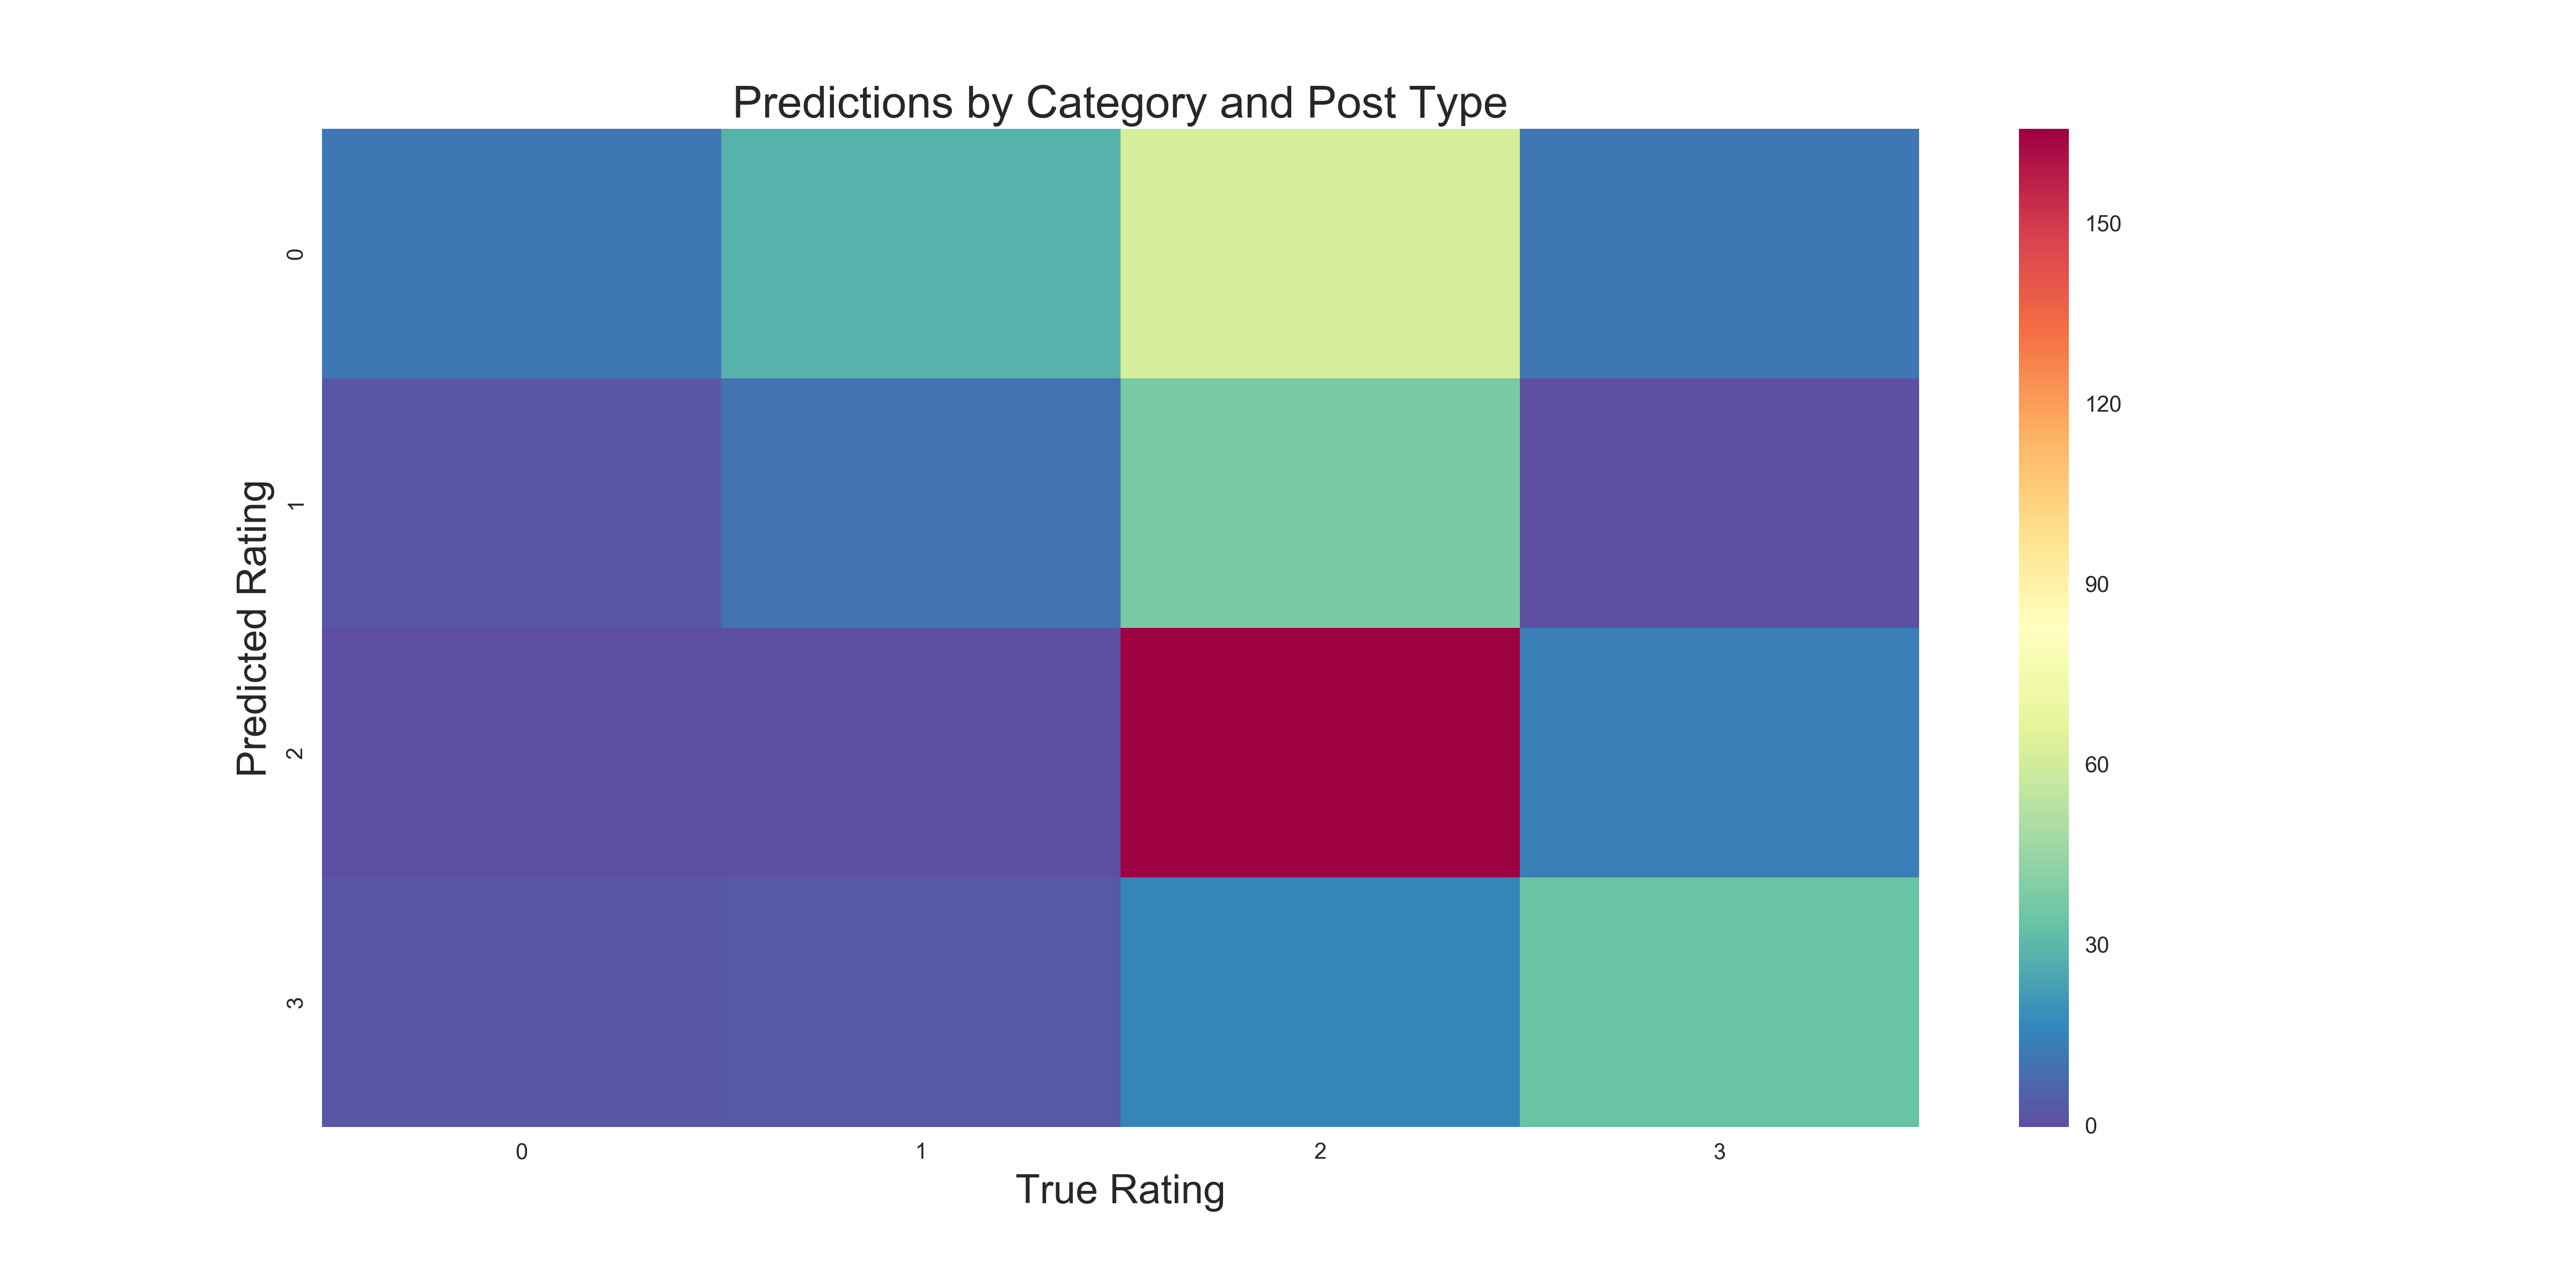
\includegraphics[width=6cm,height=4cm]{cat_predicts.png}
\end{frame}

\begin{frame}{Flagging Methods}

\begin{itemize}
\item Instead of trying to predict the exact truthfulness rating of every post, we attempt to flag potentially false posts for further investigation.
\item Measure success with sensitivity (true positives, or how many of the false posts did we catch) and specificity (true negatives, or how many of the not-false posts did we mark as not-false)
\item Use the probabilities $C_i$ obtained from the Naive Bayes model
\item Goal: High sensitivity, reasonable specificity
\end{itemize}

\end{frame}

\begin{frame}{Results}
\small
\begin{itemize}
\item Use Bayes' theorem to estimate probability that a post is false, given that we flagged it.
\item Before: 4.6\% of posts rated ``mostly false"
\item After: about 10\% of flagged posts rated ``mostly false", with no false posts left behind
\end{itemize}
\scriptsize
\begin{center}
{\renewcommand{\arraystretch}{1.5}
\begin{tabular}{|| p{0.65\textwidth} | r | r ||}

\hline \hline
\textbf{Method} & \textbf{Sensitivity} & \textbf{Specificity} \\
\hline \hline

Report false always (positive control) & 100\% & 0\% \\ 
\hline
Report false never (negative control) & 0\% & 100\% \\
\hline
Report false if ``mostly false" has highest probability & 64.28\% & 74.87\% \\
\hline
Report false if ``mostly false" or ``mixture of true and false" has highest probability & 92.85\% & 61.6\% \\
\hline
Report false if ``mostly false" is highest or second highest probability & 100.00\% & 54.92\% \\


\hline \hline
\end{tabular}
}
\end{center}
\end{frame}

\end{document}